% Tangent vs. chord vs. true arc, at small and large curvature-per-step.
% The Navigator extrapolates the TANGENT (Surface::intersect is straight-line).
% The CHORD is the secant of the arc actually flown - known only afterwards.
\documentclass[border=8pt]{standalone}
\usepackage{tikz}
\usepackage{newtxtext,newtxmath}
\usetikzlibrary{arrows.meta,positioning,calc}

\begin{document}
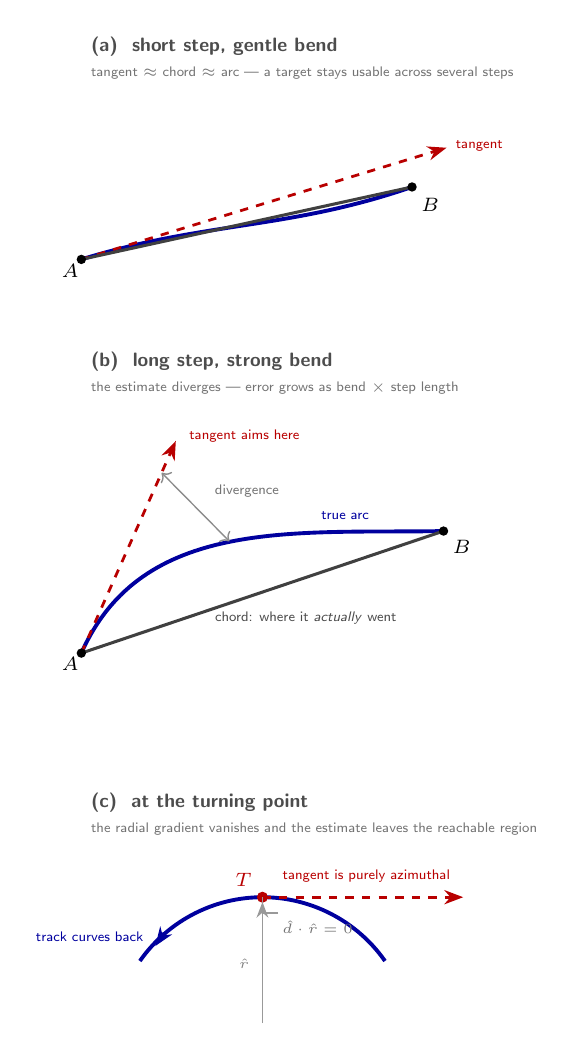
\begin{tikzpicture}[
  font=\sffamily\footnotesize,
  arc/.style={line width=1.4pt,draw=blue!62!black},
  tang/.style={line width=1.0pt,draw=red!72!black,dashed,-{Stealth[length=2.4mm]}},
  chord/.style={line width=1.1pt,draw=black!75},
  pt/.style={circle,fill=black,inner sep=1.2pt},
  lbl/.style={font=\sffamily\scriptsize},
  tny/.style={font=\sffamily\tiny},
  hd/.style={anchor=north west,align=left,font=\sffamily\scriptsize}
]

% ================= panel (a) =================
\begin{scope}
  \node[hd] at (0,2.95)
    {\textbf{\textcolor{black!70}{(a)\ \ short step, gentle bend}}\\[1pt]
     \textcolor{black!55}{\tiny tangent $\approx$ chord $\approx$ arc --- a target stays usable
     across several steps}};

  \draw[arc]  (0,0) to[out=17,in=199] (4.2,0.92);
  \draw[tang] (0,0) -- ++(17:4.85);
  \draw[chord](0,0) -- (4.2,0.92);
  \node[pt] at (0,0) {}; \node[pt] at (4.2,0.92) {};
  \node[lbl,anchor=north east,inner sep=2pt] at (0.04,0.02) {$A$};
  \node[lbl,anchor=north west,inner sep=2pt] at (4.24,0.86) {$B$};
  \node[tny,text=red!72!black,anchor=west,inner sep=2pt] at (4.68,1.44) {tangent};
\end{scope}

% ================= panel (b) =================
\begin{scope}[yshift=-50mm]
  \node[hd] at (0,3.95)
    {\textbf{\textcolor{black!70}{(b)\ \ long step, strong bend}}\\[1pt]
     \textcolor{black!55}{\tiny the estimate diverges --- error grows as bend $\times$ step length}};

  \draw[arc]  (0,0) to[out=66,in=181] (4.6,1.55);
  \draw[tang] (0,0) -- ++(66:2.95);
  \draw[chord](0,0) -- (4.6,1.55);
  \node[pt] at (0,0) {}; \node[pt] at (4.6,1.55) {};
  \node[lbl,anchor=north east,inner sep=2pt] at (0.04,0.02) {$A$};
  \node[lbl,anchor=north west,inner sep=2pt] at (4.64,1.51) {$B$};

  \node[tny,text=red!72!black,anchor=west,inner sep=3pt] at (1.26,2.76) {tangent aims here};
  \node[tny,text=black!70,anchor=north,inner sep=2pt] at (2.85,0.60) {chord: where it \emph{actually} went};
  \node[tny,text=blue!62!black,anchor=south,inner sep=2pt] at (3.35,1.62) {true arc};

  \draw[<->,draw=black!45,line width=0.5pt] (1.02,2.29) -- (1.88,1.42);
  \node[tny,text=black!55,anchor=west,inner sep=2pt] at (1.62,2.06) {divergence};
\end{scope}

% ================= panel (c) =================
\begin{scope}[yshift=-100mm]
  \node[hd] at (0,3.35)
    {\textbf{\textcolor{black!70}{(c)\ \ at the turning point}}\\[1pt]
     \textcolor{black!55}{\tiny the radial gradient vanishes and the estimate leaves the
     reachable region}};

  % arc that turns over: circle centred (2.3,0), radius 1.9
  \draw[arc] ([shift={(35:1.9)}]2.3,0) arc[start angle=35,end angle=145,radius=1.9];
  \coordinate (T) at (2.3,1.9);
  \fill[red!72!black] (T) circle (2.0pt);
  \node[lbl,text=red!72!black,anchor=south east,inner sep=2pt] at (2.24,1.96) {$T$};

  \draw[tang] (T) -- ++(0:2.55);
  \node[tny,text=red!72!black,anchor=south,inner sep=3pt] at (3.62,1.98)
    {tangent is purely azimuthal};

  % radius vector
  \draw[draw=black!40,line width=0.6pt,-{Stealth[length=2.0mm]}] (2.3,0.30) -- ($(T)-(0,0.06)$);
  \node[tny,text=black!50,anchor=east,inner sep=3pt] at (2.24,1.05) {$\hat{r}$};
  \draw[draw=black!40,line width=0.5pt] ($(T)+(0.20,-0.20)$) -- ++(-0.20,0) -- ++(0,0.20);
  \node[tny,text=black!55,anchor=west,inner sep=3pt] at (2.44,1.52) {$\hat{d}\cdot\hat{r}=0$};

  \draw[arc,-{Stealth[length=2.4mm]}] (1.05,1.44) -- (0.94,1.28);
  \node[tny,text=blue!62!black,anchor=east,inner sep=3pt] at (0.90,1.40) {track curves back};
\end{scope}

\end{tikzpicture}
\end{document}
